\documentclass[russian,english,hyperref=unicode]{beamer}

\usepackage{cmap}
\usepackage[utf8]{inputenc}
\usepackage[T1]{fontenc}
\usepackage{tikz}
\usepackage{tabularx}
\usepackage{listings}
\usepackage[russian,english]{babel}
\usepackage{mathptmx}
\usepackage{multimedia}
\usepackage{amsmath}
\usepackage{amsthm}
\usepackage{graphicx}
\usepackage{amssymb}

%LST LISTINGS
\usepackage{listings}
\usepackage{tikz,pgfplots}
%\pgfplotsset{compat=newest}
%\pgfplotsset{plot coordinates/math parser=false}

\usepackage{color}
\definecolor{gray}{rgb}{0.4,0.4,0.4}
\definecolor{darkblue}{rgb}{0.0,0.0,0.6}
\definecolor{cyan}{rgb}{0.0,0.6,0.6}

\lstset{
  showstringspaces=false,
  commentstyle=\color{gray}\upshape,
  basicstyle=\footnotesize,
  columns=flexible,
  frame=single,
  breaklines=true,
  frame=multipled
}

\lstdefinelanguage{XML}
{
  morestring=[b]",
  morestring=[s]{>}{<},
  morecomment=[s]{<?}{?>},
  stringstyle=\color{black},
  identifierstyle=\color{darkblue},
  keywordstyle=\color{cyan},
  morekeywords={xmlns,version,type}% list your attributes here
}


\usepackage[absolute,overlay]{textpos}
\usepackage[labelformat=empty]{caption}

%\usetheme{Darmstadt}...
\usetheme{default}
\usecolortheme{dove}
\usenavigationsymbolstemplate{}
\setbeamertemplate{footline}{}

 % BigIMgH
\newcommand<>{\bigimgh}[1]{
        {
                \begin{frame}
                        \begin{tikzpicture}[remember picture]
                                \node[at=(current page.center)] {
                                        \includegraphics[height=\paperheight]{#1}
                                };
                        \end{tikzpicture}
                \end{frame}
        }
}
 % BigIMg
\newcommand<>{\bigimg}[1]{
        {
                \begin{frame}
                        \begin{tikzpicture}[remember picture,overlay]
                                \node[at=(current page.center)] {
                                        \includegraphics[width=\paperwidth]{#1}
                                };
                        \end{tikzpicture}
                \end{frame}
        }
}


\author{Александр Улитин, 461 гр.}
\begin{document}
\selectlanguage{russian}

\title{ Сравнение двух подходов к повышению разрешения на примере автомобильных номеров }
\author{
  \begin{tabular}[4cm]{rl}
 Автор:                & Улитин А.~А., 461 гр. \\
 Научный руководитель: & доц.~Вахитов А.~Т.
 \end{tabular}
 }
\date{}

\begin{frame}{}
		\maketitle
\end{frame}

\section{Задача}
\begin{frame}{Задача Super-resolution}
  Задача Super resolution --- качественно повысить разрешения изображения
  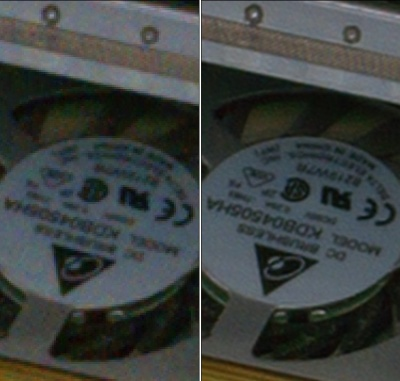
\includegraphics[height=\textheight]{content/An_example_of_super_resolution_with_still_RAW_photo.jpg}
\end{frame}

\begin{frame}{Почему это возможно}
  Для повышения разрешения используется дополнительная информация
  \begin{itemize}
    \item знание параметров съемки (размытие, движение камеры~и~т.п.)
    \item знание о типе снимаемого объекта (текст, лица, и т.п.)
    \item использование нескольких изображей, снятых с разных ракурсов
      (кадры из видео)
  \end{itemize}
  которая влияет на конечное изображение
\end{frame}

\section{Подходы}
\begin{frame}{Сравниваемые подходы}
  \begin{itemize}
    \item Couple Dictionary Training for Image Super-resolution \\
        (Jianchao Yang,Zhaowen Wang, Zhe Lin,Scott Cohen, and Thomas Huang)
      \begin{itemize}
        \item использует пару тренированных словарей
        \item восстановление по одному изображению
      \end{itemize}
    \item Superresolution of License Plates in Real Traffic Videos \\
      (K. V. Suresh, G. Mahesh Kumar, and A. N. Rajagopalan)
      \begin{itemize}
        \item для восстановление использует последовательную оптимизацию с
          регуляризаторами
        \item использует несколько изображений
      \end{itemize}
  \end{itemize}
\end{frame}

\newcommand{\inimage}[2]{
  \begin{minipage}{#1}
    \vcenter{\includegraphics[width=\columnwidth]{#2}}
  \end{minipage}
}


\section{Приведение изображений}
\begin{frame}{Несколько изображение $\rightarrow$ одно изображение}
  Для тестирования на однинаковых наборах данных из lr строились псевдо hr для
  первого алгоритма методом:
  $$ R = \frac{1}{n}\sum_{i=1}^nW^T \cdot S \cdot IMG_{lr i}$$
  $S$ --- билинейная интерполяция \\
  $W$ --- сдвиг

  \inimage{3cm}{content/imgs/append_imgs_big.jpg}
  $\to$
  \inimage{6cm}{content/imgs/combined_big.jpg}
\end{frame}

\section{PSNR}
\begin{frame}{PSNR}
$${MSE} = \frac{1}{m\,n}\sum_{i=0}^{m-1}\sum_{j=0}^{n-1} [I(i,j) -
K(i,j)]^2$$

The PSNR is defined as:
$$
\mathit{PSNR} &= 10 \cdot \log_{10} \left( \frac{\mathit{MAX}_I^2}{\mathit{MSE}} \right)
$$
\end{frame}

\section{SR1}
\begin{frame}{Исходные изображения}
  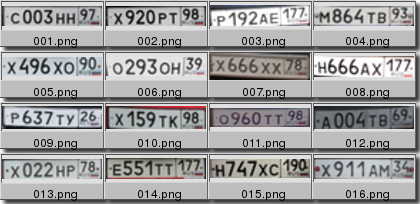
\includegraphics[width=\columnwidth]{content/out_sr1.png}
\end{frame}
\begin{frame}{Результаты подхода №1}
  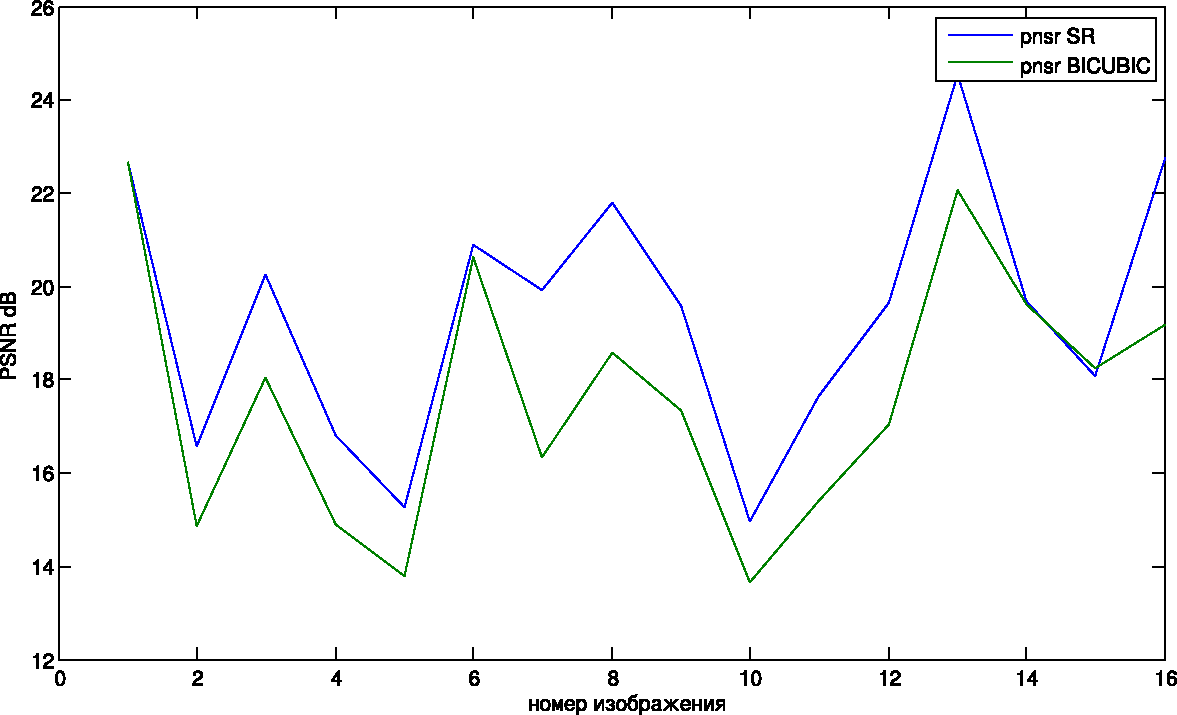
\includegraphics[width=\columnwidth]{content/pnsr_for_big_jpeg.pdf}
\end{frame}
\begin{frame}{Пример изображений}
  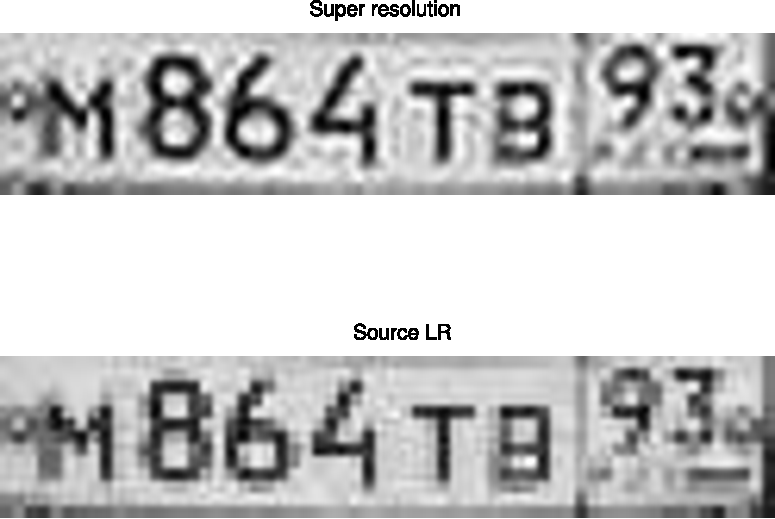
\includegraphics[width=\columnwidth]{content/compare_result_sr1.pdf}
\end{frame}

\section{XML}
%\begin{frame}{XML}
%  \textbf{XML} -- язык разметки, который определяет набор правил таких, что
%  этот формат \textmd{одинаково} хорошо читается людьми и машинами.
%
%  Простой пример
%  \lstset{language=xml}
%  \lstinputlisting{content/xmlexample1.xml}
%\end{frame}
%
%\begin{frame}{Пример чуть посложнее}
%  \lstinputlisting[language=xml]{content/xmlexample2.xml}
%\end{frame}
%
%\begin{frame}{XML+}
%  Использование XML:\\
%  XHTML, XML DOM, XSL(XSLT, XSL-FO, XPath),
%  XQuery, DTD, XSD, XLink, XPointer, SOAP, WSDL, RDF, RSS, SVG, XUL, XForms,
%  Xaml, KParts, GLADE\dots
%
%  Поговорим о:
%  \begin{itemize}
%    \item XPath
%    \item XSLT
%    \item SOAP
%  \end{itemize}
%\end{frame}
%
%\section{XPath}
%\begin{frame}[allowframebreaks=1]{XPath}
%  XPath -- язык запросов к XML.
%  \lstinputlisting[language=xml]{content/xpath.xml}
%\end{frame}
%
%\begin{frame}{XPath}
%  XPath -- синтаксис для определения частей XML документа. \\
%  Имеет более 100 встроенных функций
%
%  Пример: \\
%  \begin{itemize}
%    \item Выбрать все заголовки \\
%      /bookstore/book/title
%    \item Выбрать заголовок первой книги \\
%      /bookstore/book[1]/title \\
%    \item Заголовки книг с ценой > 35 \\
%      //book[price>35]/title
%    \item Все языки, на которых есть книги в нашем магазине \\
%      //@lang
%    \item Книги на английском языке\\
%      /bookstore/book/title[@lang='en']
%  \end{itemize}
%\end{frame}
%
%\section{XSLT}
%\begin{frame}{XSLT}
%
%  \begin{itemize}
%    \item XSL -- EXtensible Stylesheet Language.
%    \item XSL = Style Sheets for XML
%    \item XSLT -- часть XSL. XSLT определяет правила трансформации XML в любой
%      другой формат(например HTML)
%    \item Поддерживается всеми современным браузерами(и даже IE6)
%  \end{itemize}
%\end{frame}
%
%\begin{frame}{Пример}
%  Посмотрим пример XSLT
%  \begin{itemize}
%    \item showexample1
%      \begin{itemize}
%        \item простой пример с W3C
%      \end{itemize}
%    \item showexample2
%      \begin{itemize}
%        \item пример из ответа XML от vkontakte
%        \item сортировка
%        \item выборка
%        \item переменные
%      \end{itemize}
%    \item showexample3
%      \begin{itemize}
%        \item тоже самое, но с XPath
%      \end{itemize}
%  \end{itemize}
%\end{frame}
%
%\section{Web-service}
%% Введение
%\begin{frame}{Что такое Web-service}
%  \textbf{Web-service} -- программная система, которая разработана для поддержания связи с друг другом через сеть.
%
%  Программы общаются с друг другом.
%
%  \\
%  Наиболее популярные протоколы
%  \begin{itemize}
%    \item \textbf{SOAP} (Simple Object Access Protocol) -- расширение XML-RPC
%    \item \textbf{REST} (Representational State Transfer) -- концепция, манипуляция объектами на уровене CRUD
%    \item \textbf{XML-RPC} (XML Remote Procedure call) -- устарел
%    \item CORBA, GIOP, ICE, DCOM -- бинарные протоколы.
%  \end{itemize}
%\end{frame}
%
%\begin{frame}
%  \includegraphics[width=\columnwidth]{content/standards.png}
%\end{frame}
%
%\section{REST}
%\begin{frame}{REST}
%  REST -- representational state transfer. Собственно архитектура ПО для распределенных сетей, таких как веб.
%
%  Цели REST:
%  \begin{itemize}
%    \item маштабируемость компонентов
%    \item общность интерфейсов
%    \item независимое развертывание компонент
%    \item бла-бла-бла
%  \end{itemize}
%
%  Построение RESTful архитектуры:
%  \begin{itemize}
%    \item Client-server
%    \item Stateless
%    \item Cacheable
%    \item Layered system
%    \item Code on demand (optional)
%    \item Uniform interface
%  \end{itemize}
%\end{frame}
%
%
%\section{XML-RPC}
%\begin{frame}{XML-RPC}
%  Суть -- упаковываем данные в XML и передаем по HTTP.
%  \lstset{language=xml}
%  \lstinputlisting[lastline=9]{content/soap.xml}
%  \lstinputlisting[firstline=11]{content/soap.xml}
%\end{frame}
%\begin{frame}{XML-RPC}
%  Плюсы:
%  \begin{itemize}
%    \item простота(спецификация 6 страниц)
%    \item все фишки http
%  \end{itemize}
%  Минусы:
%  \begin{itemize}
%    \item много воды
%    \item воды в 4 раза больше чем в XML
%    \item лимитирован в типах
%    \item XML валидатор пропустит ошибки и пропуски в полях уровня приложения.
%  \end{itemize}
%\end{frame}
%
%\section{SOAP}
%\begin{frame}{SOAP}
%  SOAP -- расширение XML-RPC.
%  \lstinputlisting[language=xml,breaklines=true]{content/soap1.xml}
%\end{frame}
%\begin{frame}{SOAP}
%  Плюсы:
%  \begin{itemize}
%    \item возможность работать не только поверх http
%    \item сложные типы
%    \item простота
%    \item нет проблем с кодировками
%  \end{itemize}
%  Минусы:
%  \begin{itemize}
%    \item медленнее бинарных протоколов
%    \item лимитирован в типах
%    \item XML валидатор пропустит ошибки и пропуски в полях уровня приложения.
%  \end{itemize}
%\end{frame}
%
%\begin{frame}{Как это работает}
%  \begin{enumerate}
%    \item клиент читает файлы WSDL и WSML -- описание методов и типов веб-сервиса
%    \item клиент формирует запрос и отправляет на сервер (в виде XML)
%    \item сервер получает запрос и смотрит в WSDL. Тут мы можем поймать ошибки вида непереданных аргументов или опечаток
%    \item сервер нашел метод, который необходимо выполнить. Выполнил и возвращает результаты в формате, описанном в WSDL
%    \item клиент получил ответ, парсит его согласно WSDL и радуется. Или грустит, если произошла ошибка.
%  \end{enumerate}
%\end{frame}
%
%\begin{frame}{Вывод}
%  SOAP -- удобно, здорово, стандартизировано, с возможностью масштабирования (также, как и http).
%\end{frame}
%
%\begin{frame}{Мой вопрос}
%  Почему большие сайты не используют SOAP
%  \begin{itemize}
%    \item стандарт!
%    \item простой
%    \item удобно
%  \end{itemize}
%
%  А что они используют? Каждый придумал свой велосипед.
%\end{frame}
%
%\section{WCF}
%\begin{frame}{Windows Communication Foundation}
%  WCF -- фреймворк над .NET для построения сервисов.
%
%  Bindings -- привязка к какому либо интерфейсу общения (http, tcp, message queues\ldots)
%
%\end{frame}
%
%\bigimgh{content/wcf.png}
%
%
%\section{Example}
%\begin{frame}{Пример}
%  Рассмотрим пример приложения:
%
%  Мы хотим создать сервис, который позволял бы нам получить список процессов, запущенных на компьютере
%  \vspace{1em}\\
%  \textbf{Технологии:} .NET 4.0, WCF, Visual Studio 2012, Vim
%\end{frame}
%\section{Google}
%\begin{frame}{На погуглить}
%  \begin{itemize}
%    \item XML, JSON, YAML
%    \item технологии XML
%      \begin{itemize}
%        \item XSLT, XPath, XSL
%        \item DTD, XSD
%        \item SVG
%        \item W3C XML
%      \end{itemize}
%    \item Web-services
%      \begin{itemize}
%        \item SOAP
%        \item REST
%        \item Windows Communication Foundation, RMI, Java EE, JMS
%      \end{itemize}
%  \end{itemize}
%\end{frame}


\end{document}
